%++++++++++++++++++++++++++++++++++++++++
% Don't modify this section unless you know what you're doing!
\documentclass[letterpaper,12pt]{article}
\setlength{\parindent}{4ex}
\setlength{\parskip}{1ex}

\usepackage{graphicx}
\usepackage{indentfirst}
\usepackage{tabularx} % extra features for tabular environment

\usepackage{caption} % Spacing between caption (title) and actual table
\captionsetup[table]{skip=10pt}

\usepackage{amsmath}  % improve math presentation
\usepackage{graphicx} % takes care of graphic including machinery
\usepackage[margin=1in,letterpaper]{geometry} % decreases margins
\usepackage{cite} % takes care of citations
\usepackage[final]{hyperref} % adds hyper links inside the generated pdf file
\hypersetup {
	colorlinks=true,       % false: boxed links; true: colored links
	linkcolor=blue,        % color of internal links
	citecolor=blue,        % color of links to bibliography
	filecolor=magenta,     % color of file links
	urlcolor=blue         
      }
      \setcounter{tocdepth}{3}

\usepackage{pgfplots}      


% ++++++++++++++++++++++++++++++++++++++++

\begin{document}

\title{CS 7641 Machine Learning \\
		\ Assignment 1 }
\author{David Yun}
\date{September 23, 2018}
\maketitle

\begin{abstract}
  The implementation, and basic fundamentals behind the following Machine Learning Algorithms will be discussed in detail:  
  \begin{enumerate}
    \item Decision trees with some form of pruning
    \item Neural Networks
    \item Boosting
    \item Support Vector Machines (SVM)
    \item k-Nearest Neighbors (kNN)
      
    \end{enumerate}

    For this assignment, Python is used, along with the necessary libraries associated within each topic.  The full code files are available on github\footnote{David Yun's Github: \url{https://github.com/tree-fiddy/Assignment_1}}
    Please refer to the README.txt file for concise instructions on how to run the files associated with each aforementioned algorithms.  The full README.md file will guide a reader on how to use the files to better understand the objectives of this Assignment.  

\end{abstract}

\tableofcontents

\section{Decision Trees}

The implementation of Decision Trees was borrowed from my previous coursework in CSE6242 (Data Visualization) with minor tweaks.  

\subsection{Dataset and Code}
The dataset provided in this directory is the UCI Credit Approval Dataset\footnote{UCI Credit Approval Data Set: \url{http://archive.ics.uci.edu/ml/datasets/credit+approval}}.  Some small adjustments were made to the dataset, such as removing rows where data was missing.  

\subsection{Analysis}
The accuracy of our decision tree relies on our tolerance for pre-pruning.  In essence, one must specify \emph{when} to stop growing the tree.  On one extreme, we can set a condition to stop growing the tree once we reach a \emph{pure\footnote{A leaf is said to be ``pure'' if the leaf contains homogenous labels.  By extension, this equates to a situation where Entropy equals 0.}} leaf.  However, this will likely make the tree longer than need be.  A more depth-restrictive approach is to set an arbitrary threshold for Entropy in our Decision Tree, where we will halt further node and leaf generation if the current node produces leaves with Entropy values less than our specified threshold.  The performance of our decision tree, while varying \text{threshold levels} is highlighted in Table \ref{table:PrePruningTable}.

\begin{table}[htb]
  \caption{Pre-Pruning Spec Performance (forest size = 50)}
  \label{table:PrePruningTable}
  \centering
  \begin{tabular}{|c|c|c|}
  
    \hline
    \hline
    \multicolumn{1}{c}{Entropy Threshold}
    &  \multicolumn{1}{c}{Model Accuracy} \\
    \cline{1-2}
    0.0 & 0.86 \\
    \cline{1-2}
    0.1 & 0.86 \\
    \cline{1-2}
    0.2 & 0.60 \\
    \cline{1-2}
    0.3 & 0.57 \\
    \cline{1-2}
    0.4 & 0.55 \\
    \cline{1-2}
    0.5 & 0.55 \\
    \cline{1-2}
    0.6 & 0.54 \\
    \cline{1-2}
    0.7 & 0.54 \\
    
    
    \cline{1-2}
  \end{tabular}
\end{table}

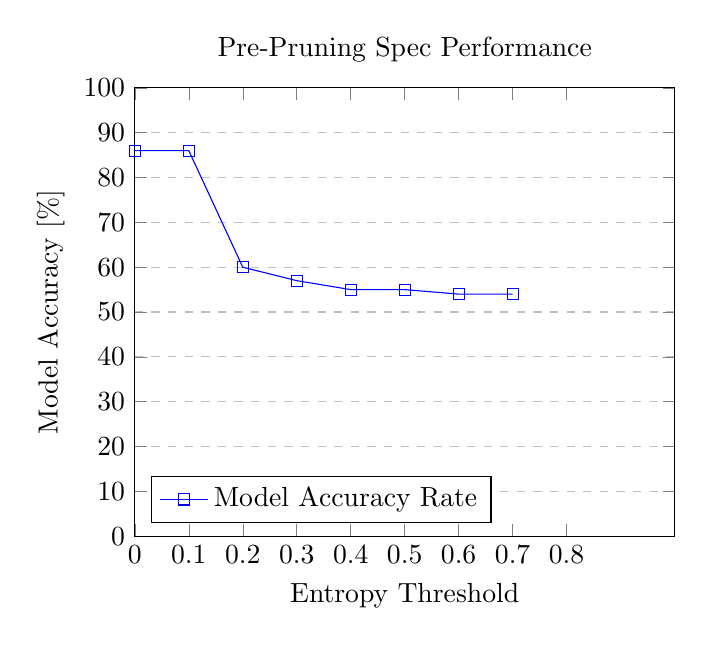
\begin{tikzpicture}
  \begin{axis} [
      title = {Pre-Pruning Spec Performance},
      xlabel = {Entropy Threshold},
      ylabel = {Model Accuracy [\%]},
      xmin = 0, xmax = 1,
      ymin = 0, ymax = 100,
      xtick={0,0.1,0.2,0.3,0.4,0.5,0.6,0.7,0.8},
      ytick={0,10,20,30,40,50,60,70,80,90,100},
      legend pos = south west,
      ymajorgrids=true,
      grid style = dashed
      ]
      \addplot[
      color = blue,
      mark = square,
      ]
      coordinates {
    (0.0,86)(0.1, 86)(0.2, 60)(0.3,57)(0.4,55)(0.5,55)(0.6,54)(0.7,54)
    };
    \legend{Model Accuracy Rate}
 
\end{axis}
\end{tikzpicture}

As you can see, the model's accuracy reached an asymptote of around 50\% accuracy, which indicates that setting a higher threshold for Entropy renders this model's efficacy no better than a coin flip.  Thus, setting a pre-pruning specification is quite important here.  More notable is the fact that using the extreme case where Entropy must equal 0 before considering the tree complete yielded the same results as a 0.1 threshold.  However, computation times were slightly longer for this case, as more nodes had to be constructed until the threshold was met.  While in our dataset, it wasn't a huge factor, this is an important consideration one should make when building models on much larger data.  When the efficacy/accuracy of a model isn't compromised, any measures to speed up performance is a welcomed consideration.  

\section{Dataset 2:  Credit Bureau Data}
This dataset includes the following:

\begin{itemize}
\item First \& Last \& Middle names
\item Marital Status
\item Sex
\item Birth Year
\item Whether they owned real estate
\item Current City
\item Email Domain
\item List of Monthly Payment status over 5 years for various tradelines
\end{itemize}

Like the alumni magazine dataset, this dataset can also be used for clusting and/or classification.  Again, by itself, it's not useful beyond labeling a particular customer among a range of financial well-being compared to his/her peers.  Perhaps, this dataset can be solely used for Prospecting (ie. obtaining a list of potential customers, and sending marketing offers).  However, we will keep this paper limited in scope to leveraging data to understand existing customers, rather than prospecting potential customers.  

\section{Dataset 3: Company Web Site Tracking Data}
This dataset includes the following:

\begin{itemize}
\item Title
\item First \& Last \& Middle (initial) names
\item Credit Card Type
\item Credit Card Number
\item List of products purchased in the past, with date of purchase and ship-to-address
\item Which web pages the person looked at
\item How long the person spent on each page
\item What the person clicked on each page
\item Estimate of how long the user's eyes spent on each page viewed (through camera)
\end{itemize}

This dataset is more worthwhile for the Company.  It gives direct actionable response variables (Products purchased, web page landing statistics, click through rates...etc.).

Given this dataset alone, the company can use \emph{Graph Theory} to understand the path in which a set of customers take to final purchase in order to optimize the customer experience to decreases the abandonment rate of online shopping carts.

Shopping fatigue can exist even through online channels.  The plethora of buying decisions is not immune to online retail, and time spent hopping around products can be physically exhausting.  In a literal sense, batteries can be exhausted while shopping, increasing the likelihood that shopping carts will be abandoned.  To combat this, our company can look at the paths our average customer takes when making purchases.  Perhaps there are too many forms being filled out to finalize a purchase, aiding in shopping fatigue.

The real value in this dataset lies on cross-selling potential.  Again, \emph{Graph Theory} can be used to determine cliques of items that tend to be included in a customer's basket of goods.  By first identifying these cliques of items, a recommendation engine can be leveraged to increase sales while a customer is on the check out page.  Furthermore, the retailer can investigate why certain products are not purchased together.  For example, if retailers see a spike in peanut butter sales, but not a corresponding increase in, say, jelly sales, perhaps the retailer is charging too much for jelly.

\section{Datasets Combined}
The value of the datasets can be maximized by integrating them to obtain insights that a single dataset won't provide.  While there aren't unique identifiers that can easily link the 3 datasets, one can achieve a reasonable amount of success in the following manner:

\begin{table}
  \caption{Alumni-Credit Data Merge}
  \centering
  \begin{tabular}{ |r|c|c|}
    \multicolumn{1}{c}{Alumni Magazine}
    &  \multicolumn{1}{c}{Credit Bureau} \\
    \cline{1-2}
    First and Last Names & First and Last Names \\
    \cline{1-2}
    Email Domain & Email Domain \\
    \cline{1-2}
    Current City & Current City \\
    \cline{1-2}
  \end{tabular}
\end{table}

\begin{table}
  \caption{Alumni-Credit-Company Data Merge}
  \centering
  \begin{tabular}{ |r|c|c|}
    \multicolumn{1}{c}{Alumni-Credit Merged Data}
    &  \multicolumn{1}{c}{Company Data} \\
    \cline{1-2}
    First and Last Names & First and Last Names \\
    \cline{1-2}
    Current City & Ship-to-City \\
    \cline{1-2}
  \end{tabular}
\end{table}

Notice that the company collected data only has City, First and Last name as common fields to be merged on.  This reduces the reliability of the full dataset.  However, we can still make a reasonable guess at the correct linkages, and assume Name + City is a unique identifier for our purpose here.

The data made available to us is immediately useful for the purpose of segmenting our existing customers.  Using kMeans clustering, we can create distinct groupings of our existing customers and gather insights on key variables likely to predict shopping behavior.

Moreover, the combined datasets can be used for \emph{prospecting} purposes.  It is likely that level of education, and specifically, institution attended, are predictors of purchasing behavior.  In order to test that, our combined dataset will allow us to see if it's worth pursuing/expanding an education demographic to increase sales.  There are too many combinations of variables that can be analyzed to ascertain clusters, so I won't go into it here.

Last but not least, we can apply optimization models to determine which demographic we \emph{should} be targeting at a particular time of day, month, or year.  For example, with our purchased datasets, we may have determined that wives without a college education, who are current on their mortgages, who have high credit card debt, are very active on our retailer's website during 2 P.M.  We can serve ads heavily to this demographic at the right times.  Furthermore, we can tell our advertising partners to serve the bulk of our ads across all platforms where it is likely that our potential customers are making buying decisions around the same time every day, or particular time in the month.  Our optimization model's \emph{objective function} will be to \textbf{Maximize sales to people who are likely to restrain from making purchases in the middle of the day}.  

Our \emph{variables} will be:

\begin{itemize}
\item Level of Education dummy variables
\item Real estate owner dummy variable
\item Marital Status
\item Gender
\item Month dummy variables
\item City
\item ``Lurker'' indicator variable
\item Frequent Visitor indicator variable
  \item Penchant to Purchase, but witholding indicator variable
\end{itemize}

In our problem, we want to constrain our optimization model to hone in our demographic by including the following constraints:

\begin{itemize}
\item Frequent Visitor
\item Lurker (person spends 30 min each visit)
\item Penchant to purchase (eyes gaze on a product for more than a minute)
\end{itemize}

Using these constraints, we are likely to pick up customers who really are making a conscientious effort \emph{not} to buy whatever the customer is looking at.  
    

This optimization model will determine the most optimum demographic to pursue the right demographic to target our advertisements to.  Implicit in our optimization model is the assumption that we are selling luxury goods- items that the average consumer can do without.  Our goal is to first identify which cohorts are likely to yearn for an item.  Then, our next goal will be to find the perfect promotion strategy (15\%, 20\%, 30\%...etc. discount, Buy 1 get 1 Free, Email abandoned cart reminders...etc.) to entice the customer to finally make a purchase. 
       

\end{document}
